%% Placeholder for chapter on SVD
%% Placeholder for chapter on SVD
\section{The Singular Value Decomposition(SVD)}

Let's review our previous results before starting the SVD part.

\subsection{Eigen-decomposition}

For any $A\in \reals^{n\times n}$ that is diagonalizable,  we can express $A$ as 
\begin{equation*}
A = U\Lambda U^{-1}
\end{equation*}

$U$: $n$ by $n$ invertiable matrix of linear independent eigenvectors $\in \mathbb{C}^n$, that is, each column of $U$ is an eigenvector of $A$.

$\Lambda$: a diagonal matrix whose diagonal entries are eigenvalues of $A$, and $\lambda_i\in \mathbb{C}$.


\subsection{Spectral decomposition}

For any $n$ by $n$ symmetric matrix $A$, we can express $A$ as
\begin{equation*}
A = U\Lambda U^T
\end{equation*}

$U$: Orthogonal matrix ($\perp$ \& normalized) $U^{(i)}\in \Re^n$;

$\Lambda$: Diagonal matrix of $\lambda_i \in \Re$.



\subsection{Singular Value Decomposition(SVD)}

For any matrix $A\in \reals^{m\times n}$, we can be expressed $A$ as 
\begin{equation*}
A =U\tilde{\Sigma} V^T
\end{equation*}

$U\in \reals^{m\times m}$: An orthogonal matrix, so $UU^T =U^TU = I_m$

$V\in \reals^{n\times n}$: An orthogonal matrix, so $VV^T = V^TV =I_n$

$$\tilde{\Sigma} = 
\left[
\begin{matrix}
\Sigma & \textbf{0}\\
\textbf{0}&\textbf{0}
\end{matrix}
\right]\in \reals^{m\times n}
$$

where $\Sigma = diag(\sigma_1,...,\sigma_r)> 0$.


Comments on SVD: 
\begin{itemize}
	\item Inherits $\perp$ matrices of spectral decomposition and all $\lambda_i$ are real.
	\item Generalizes eigen-decomposition and spectral decomposition to a non-square matrices.
	\item Lose the property of direction invariance of eigen-decomposition.
\end{itemize}


\vspace{0.5cm}
\begin{example}
	Let's consider an example, $y = Ax = U\tilde{\Sigma} V^Tx$, and see how these matrices impose influences on a vector $x$(refer to the figures on the r.h.s)
	$$U = 
	\left[
	\begin{matrix}
	\frac{1}{\sqrt{3}}&\frac{1}{\sqrt{2}} & \frac{1}{\sqrt{6}}\\
	\frac{1}{\sqrt{3}}&-\frac{1}{\sqrt{2}} & \frac{1}{\sqrt{6}}\\
	\frac{1}{\sqrt{3}}&0 & -\frac{2}{\sqrt{6}}
	\end{matrix}
	\right]
	 ,
	\tilde{\Sigma} = 
	\left[
	\begin{matrix}
	2&0\\
	0&0\\
	0&0
	\end{matrix}
	\right] 
	,
	V = 
	\left[
	\begin{matrix}
	-\frac{1}{\sqrt{2}}&\frac{1}{\sqrt{2}}\\
	\frac{1}{\sqrt{2}}&\frac{1}{\sqrt{2}}
	\end{matrix}
	\right] 
	,
	A = 
	\left[
	\begin{matrix}
	-\frac{2}{\sqrt{6}}&\frac{2}{\sqrt{6}}\\
	-\frac{2}{\sqrt{6}}&\frac{2}{\sqrt{6}}\\
	-\frac{2}{\sqrt{6}}&\frac{2}{\sqrt{6}}
	\end{matrix}
	\right]
	$$
	
$ 1) x = 
	\left[
	\begin{matrix}
	1\\
	0
	\end{matrix}
	\right]
$
	\begin{marginfigure}
		\centering
		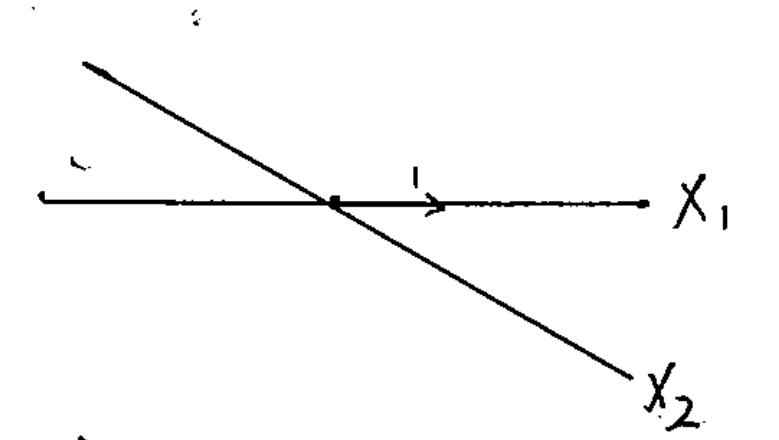
\includegraphics[width=1.8in,height=1.8in]{figures/ch05/figure1_a.jpg}
		%\caption{This is an inserted JPG graphic} 
		%\label{fig:graph} 
	\end{marginfigure}


$ 2) w = V^Tx = 
	\left[
	\begin{matrix}
	-\frac{1}{\sqrt{2}}\\
	\frac{1}{\sqrt{2}}
	\end{matrix}
	\right]
$
	

$ 3) z = \Sigma w = 
	\left[
	\begin{matrix}
	-\frac{1}{\sqrt{2}}\\
	0\\
	0
	\end{matrix}
	\right]
$
	
	\begin{marginfigure}
		\centering
		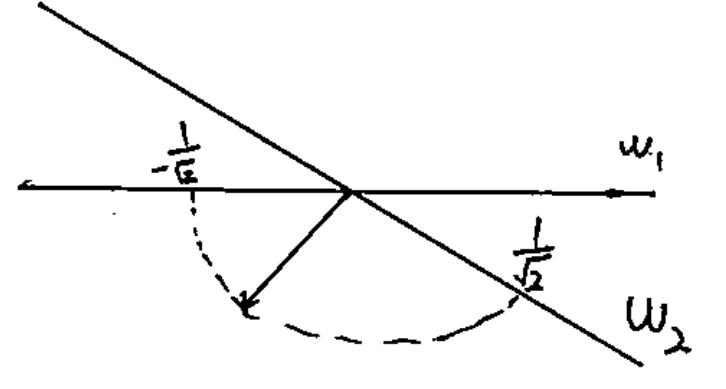
\includegraphics[width=1.8in,height=1.8in]{figures/ch05/figure1_b.jpg}
		%\caption{This is an inserted JPG graphic} 
		%\label{fig:graph} 
	\end{marginfigure}

	\begin{marginfigure}
		\centering
		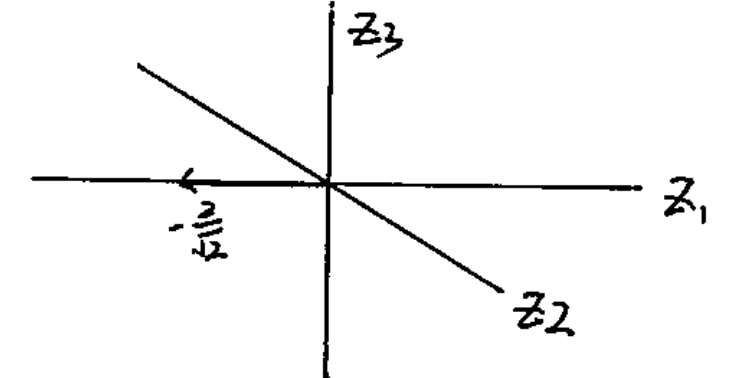
\includegraphics[width=1.8in,height=1.8in]{figures/ch05/figure1_c.png}
		%\caption{This is an inserted JPG graphic} 
		%\label{fig:graph} 
	\end{marginfigure}

$ 4) y = Uz =  
	\left[
	\begin{matrix}
	-\frac{2}{\sqrt{6}}\\
	-\frac{2}{\sqrt{6}}\\
	-\frac{2}{\sqrt{6}}
	\end{matrix}
	\right]
$
	\begin{marginfigure}
		\centering
		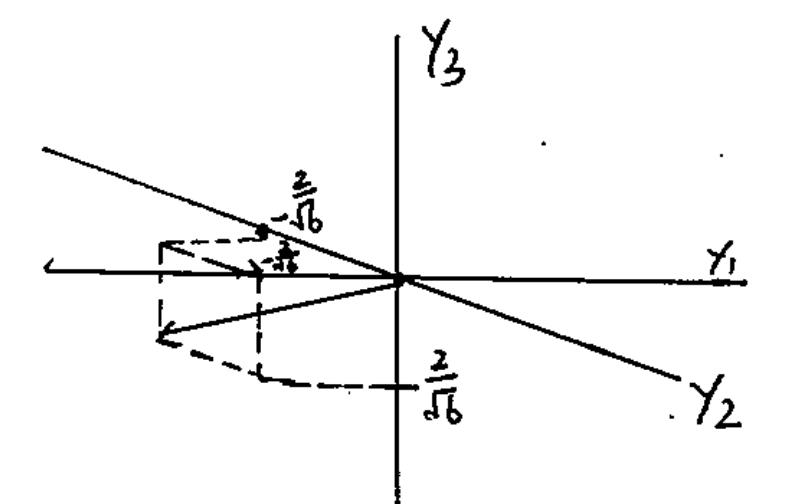
\includegraphics[width=1.8in,height=1.8in]{figures/ch05/figure1_d.jpg}
		%\caption{This is an inserted JPG graphic} 
		%\label{fig:graph} 
	\end{marginfigure}
	

\end{example}

This example and the figures show that the SVD of a matrix $A$ has lost the property of direction invariance, compared to the eigen-decomposition.



\vspace{2cm}
\subsection{Computing SVD}
The idea of singular value decomposition(SVD) follows from eigen-decomp of $A^TA$ and $AA^T$, since both of these two matrices are symmetric, so the spectral theorem is applicable(i.e., $A^TA$ and $AA^T$ can be orthogonally diagonalize). 

Let $A$ be an $m$ by $n$ matrix. First, we let $\lambda_i$ denote eigenvalues of the symmetric matrix $A A^T$ (or of matrix $A^T A$), and arrange these eigenvalues in a decreasing order, that is, $\lambda_1\geq \lambda_2\geq \cdots \geq \lambda_m$(there are $n$ eigenvalues if we consider $A^TA$). We define the singular value of a matrix $A$ as the square root of the eigenvalues and arrange them in a decreasing order as well, i.e., $\sigma_i=\sqrt{\lambda_i}$ and suppose we have $r$ singular values that are positive, so $\sigma_1\geq \sigma_2\geq \cdots \geq \sigma_r>0$.


By spectral theorem, we write out $U$ and $V$ as (note that $\rank(A)=r$):
$$ U =   
\left[
\begin{matrix}
U^{(1)} & ... & U^{(r)} & U^{(r+1)} & ... & U^{(m)}
\end{matrix}
\right] =
\left[
\begin{matrix}
U_r & U_{mr}
\end{matrix}
\right]
$$

$$ V =   
\left[
\begin{matrix}
V^{(1)} & ... & V^{(r)} & V^{(r+1)} & ... & V^{(n)}
\end{matrix}
\right] =
\left[
\begin{matrix}
V_r & V_{nr}
\end{matrix}
\right]
$$

Thus,
\begin{align*}
AA^T &= U\tilde{\Sigma} V^TV\tilde{\Sigma}^TU^T\\
&=
\begin{bmatrix}
\mathcal{U}_r & \mathcal{U}_{mr}
\end{bmatrix}
\begin{bmatrix}
\Sigma & \textbf{0}\\
\textbf{0}&\textbf{0}
\end{bmatrix}
\begin{bmatrix}
\Sigma & \textbf{0}\\
\textbf{0}&\textbf{0}
\end{bmatrix}
\begin{bmatrix}
\mathcal{U}_r^T\\
\mathcal{U}_{mr}^T
\end{bmatrix}\\
&
=\begin{bmatrix}
\mathcal{U}_r & \mathcal{U}_{mr}
\end{bmatrix}
\begin{bmatrix}
\Sigma^2 & \textbf{0}\\
\textbf{0}&\textbf{0}
\end{bmatrix}
\begin{bmatrix}
\mathcal{U}_r^T\\
\mathcal{U}_{mr}^T
\end{bmatrix}\\
&= \sum^r_{i=1}(\sigma_i)^2u^{(i)}u^{(i)^T}\\
&= \sum^m_{i=1}(\sigma_i)^2u^{(i)}u^{(i)^T}
\end{align*}

We may noticed that the vector $u^{(k)}$ is $k^{th}$ eigenvector of $AA^T$ by showing that
\begin{align*}
(AA^T)u^{(k)} 
& = \sum^m_{i=1}\sigma_i^2u^{(i)}(u^{(i)})^Tu^{(k)}\\
& = \sum^m_{i=1}\sigma_i^2 \mathbb{1}_{i=k} u^{(i)} \\
& = \sigma^2_ku^{(k)}\\
& = \lambda_k u^{(k)}
\end{align*}
where $\lambda_k$ is the k-th eigenvalue of $AA^T$, and the indicator function comes from the orthogonality of matrix $\mathcal{U}$.

The same logic can be applied to $A^TA$ and shows that $v^{(k)}$ is $k^{th}$ eigenvector of $A^TA$.

Accordingly, we have already to know how to obtain he SVD  of a matrix.


We summarize the procedure that how we compute the SVD of a matrix $m$ by $n$ matrix $A$ as follows

1) Singular values: Compute eigenvalues of $AA^T$ or $A^TA$, and to find the $r$ positive singular values $\sigma_i = \sqrt{\lambda_i(A^TA)}$, so we have the matrix $\tilde{\Sigma}$ with diagonal entries are these positive singular values and other entries are zero.

%$x^TA^TAx = w^Tw =\Vert w\Vert^2$

2) Right-Singular vectors $v^{(i)}$: Find the eigenvectors of $A^TA$, so we have an $n$ by $n$ orthogonal matrix $V$.

3) Left-Singular vectors $u^{(i)}$: Find the eigenvectors of $AA^T$, so we have an $m$ by $m$ orthogonal matrix $\mathcal{U}$.

4) Write down the expression $A = \mathcal{U} \tilde{\Sigma} V^T$.

\vspace{0.5cm}

\subsection{Bases for Fundamental Subspaces}
Let's consider arbitrary $x\in \reals^n$, 
\begin{align*}
Ax 
&= U\tilde{\Sigma} V^Tx\\
&= 
\begin{bmatrix}%
U_r & U_{mr}
\end{bmatrix}
\begin{bmatrix}%
\Sigma & \textbf{0}\\
\textbf{0}& \textbf{0}
\end{bmatrix}
\begin{bmatrix}%
V_r^T\\
V_{mr}^T
\end{bmatrix}x\\
&= 
\begin{bmatrix}%
U_r & U_{mr}
\end{bmatrix}
\begin{bmatrix}%
\Sigma\\
\textbf{0}
\end{bmatrix}
\begin{bmatrix}%
V_r^T
\end{bmatrix}x\\
&=
U_r \Sigma V_r^T x\\
&= \Sigma^r_{i=1}\sigma_iu^{(i)}(v^{(i)})^Tx
\end{align*}
\\

The above equalities show us that we have lost all components of $x$ along $v^{(i)}$ directions when $r+1 \leq i \leq n$, i.e., columns of $V_{nr}$. We summarize the results as follows:

(1) All direction in output are in span $\{u^{(1)} ,..., u^{(n)}\}$

(2) Columns of $V_{r}$ provide basis for $R(A^T)$

(3) Columns of $V_{nr}$ provide basis for $N(A)$.

(4) Columns of $U_r$ provide basis for $R(A)$.

(5) Columns of $U_{mr}$ provide basis for $N(A^T)$



%2) Consider arbitrary $x\in \Re^n$

%\begin{align*}
%A &= \mathcal{U}\tilde{\Sigma}V^r\\
%&= 
%\begin{bmatrix}
%\mathcal{U}_r & \mathcal{U}_{mr}
%\end{bmatrix}
%\begin{bmatrix}
%\Sigma & \mathbf{0}\\
%\mathbf{0} & \mathbf{0}
%\end{bmatrix}
%\begin{bmatrix}
%V_r^T\\
%V_{nr}^T
%\end{bmatrix}\\
%&= 
%\begin{bmatrix}
%\mathcal{U}_r & \mathcal{U}_{mr}
%\end{bmatrix}
%\begin{bmatrix}
%\Sigma \\
%\mathbf{0} & 
%\end{bmatrix}
%\begin{bmatrix}
%V_r^T
%\end{bmatrix}\\
%&= \mathcal{U}_r\Sigma V_r^T\\
%\end{align*}

%$$\mathcal{U}_r^TAV_r &= \mathcal{U}_r^T(\mathcal{U}_r\Sigma V_r^T)V_r = \Sigma$$


%\begin{align*}
%A &= \mathcal{U}_r\Sigma V_r^T \\
%&= \sum^r_{i=1}\mathcal{U}^{(i)}(V^{(i)})^T\sigma_i\\
%&= \sigma_1\mathcal{U}^{(1)}V^{(1)^T}+ \sigma_2\mathcal{U}^{(2)}V^{(2)^T}
%\end{align*}

%\begin{equation*}
%\sigma_1\mathcal{U}V^{(1)^T} = 
%\begin{bmatrix}
%\sigma_1V_1^{(1)}\mathcal{U}^{(1)} & \sigma_1V_2^{(1)}\mathcal{U}^{(1)} & ... & %\sigma_1V_n^{(1)}\mathcal{U}^{(1)}
%\end{bmatrix}
%\end{equation*}



\subsection{Condition number}
Most numerical computations involving an equation $Ax = b$ are as reliable as possible when the SVD of $A$ is used. The two
orthogonal matrices $U$ and $V$ do not affect lengths of vectors or angles between vectors. Any possible instabilities in numerical calculations are identified in $\Sigma$. If the singular values of $A$ are extremely large or small, roundoff errors are almost inevitable, but an error analysis is aided by knowing the entries in $\Sigma$ and $V$.

If $A$ is an invertible $n$ by $n$ matrix, then the ratio $\sigma_1/\sigma_n$ of the largest and smallest singular values gives the \textbf{condition number} of $A$ (Actually, a “condition number” of $A$ can be computed in several ways).

Let's consider $Ax = b$ when $A$ is invertible. We solve for $x$ and obtain that $x = A^{-1}b$. What if $b = b_r + e$? how much does solution change (let's take $b$ as the true value and $e$ as the round-off error here) ?

Now, our solution is $\hat{x} = A^{-1}b_r + A^{-1}e$.

\begin{equation*}
\frac{\frac{\Vert A^{-1}e\Vert}{\Vert A^{-1}b_r\Vert}}{\frac{\Vert e\Vert}{\Vert b\Vert}} = \frac{\Vert A^{-1}e\Vert_2}{\Vert e\Vert_2} \frac{\Vert b\Vert_2}{\Vert A^{-1}b\Vert_2}
\end{equation*}

\begin{align*}
max_{e,b\neq 0} \, \frac{\Vert A^{-1}e\Vert}{\Vert e\Vert} \frac{\Vert b\Vert}{\Vert A^{-1}b\Vert} 
&= \left[\max_{e\neq 0}\, \frac{\Vert A^{-1}e\Vert}{\Vert e\Vert}\right]\left[max_{b\neq 0}\, \frac{\Vert b\Vert}{\Vert A^{-1}b\Vert}\right]\\
&= \frac{\sigma_{\max}(A^{-1})}{\sigma_{\min}(A^{-1})}\\
&= \frac{\frac{1}{\sigma_n}}{\frac{1}{\sigma_1}}\\
&= \frac{\sigma_1}{\sigma_n}\\
&= \frac{\sigma_{\max}(A)}{\sigma_{\min}(A)}\\
&= K(A)
\end{align*}
where $K(A)$ is defined as the condition number of matrix $A$.

\begin{marginfigure}
	\centering
	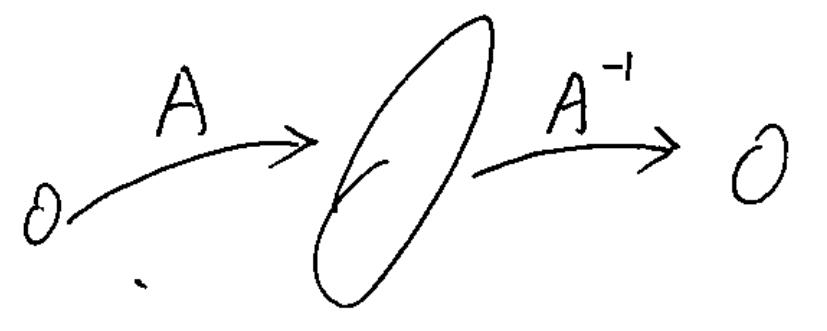
\includegraphics[width=2in,height=2in]{figures/ch05/figure2.jpg}
	%\caption{This is an inserted JPG graphic} 
	%\label{fig:graph} 
\end{marginfigure}

Note that, by the SVD of $A^{-1}$ we have
\begin{align*}
A^{-1} 
&= (\mathcal{U}\Sigma V^T)^{-1} \\
&= V\Sigma^{-1}\mathcal{U}^T\\
&= V
\begin{bmatrix}
\frac{1}{\sigma_1} & &\\
& \ddots & \\
& & \frac{1}{\sigma_n}
\end{bmatrix}
<<<<<<< HEAD
\mathcal{U}^T
\end{align*}

and by the definition of Rayleigh Quotients we have 
$$\sigma_{max}(A^{-1}) = \frac{1}{\sigma_n}$$
$$\sigma_{min}(A^{-1}) = \frac{1}{\sigma_1}$$

\subsection{Reduced SVD and Pseudo inverse}
When matrix $\tilde{\Sigma}$ contains a zero row (or column) vector, we may have a simplified expression compared to the original SVD, namely, reduced SVD:
\begin{align*}
A &= \mathcal{U}\tilde{\Sigma}V^r\\
&= 
\begin{bmatrix}
\mathcal{U}_r & \mathcal{U}_{mr}
\end{bmatrix}
\begin{bmatrix}
\Sigma & \mathbf{0}\\
\mathbf{0} & \mathbf{0}
\end{bmatrix}
\begin{bmatrix}
V_r^T\\
V_{nr}^T
\end{bmatrix}\\
&= \mathcal{U}_r\Sigma V_r^T\\
\end{align*}
Noticed that the diagonal entries of matrix $\Sigma$ are non-zero, so we may have the pseudo inverse(i.e., Moore–Penrose inverse) of matrix $A$, which is given by
$$A^{+} = V_r \Sigma^{-1} \mathcal{U}_r^T $$


\subsection{SVD and matrix norms}
Recall the definition of matrix norms (Frobenius norm), it turns out that there is connection between Frobenius norm and the singular values:
\begin{align*}
\Vert A\Vert_F^2 
&=\sum_i \sum_j	a_{ij}^2\\
&=\trace(A^TA)\\
&=\trace(V\tilde{\Sigma}^T U^T U \tilde{\Sigma} V^T)\\
&=\trace(V \tilde{\Sigma}^T \tilde{\Sigma} V^T)\\
&=\trace(V V^T \tilde{\Sigma}^T \tilde{\Sigma})\\
&=\trace(\tilde{\Sigma}^T \tilde{\Sigma})\\
&=\trace(\tilde{\Sigma}^2)\\
&=\sum_{i=1}^{r} \sigma_i^2
\end{align*}

That is, the Frobenius norm of $A$ equals to the sum of the square of positive singular values.
=======
\mathcal{U}^T\\
\sigma_{max}(A^{-1}) = \frac{1}{\sigma_n}\\
\sigma_{min}(A^{-1}) = \frac{1}{\sigma_1}
\end{align}

\begin{equation*}
max_{e\neq 0} \frac{||A^{-1}e||}{||e||} =\sigma_{max}(A^{-1})
\end{equation*}

$\rightarrow$ Rayleigh Quatients

General matrix $A\in \Re^{m\times n}$

\begin{equation*}
max_{x\neq 0} \frac{||Ax||}{||x||} = max_x\frac{||Ax||^2}{||x||^2} = max_x\frac{x^TA^TAx}{x^Tx}
\end{equation*}

By Thm4.3: 

\begin{equation*}
\lambda_{min}(A^TA)\leq \frac{x^T(A^TA)x}{x^Tx}\leq \lambda_{max}(A^TA)
\end{equation*}

where 
\begin{equation}
\label{eq6}
\lambda_{min}(A^TA)=\left\{
\begin{aligned}
\sigma_{min}(A)^2 & , & rank(A) = n \\
0 & , & otherwise
\end{aligned}
\right.
\end{equation}

Then we can have:

\begin{align*}
arg\, max_x\frac{||Ax||}{||x||} &= arg\, max_x||A\frac{x}{||x||}||\\
&= arg\, max_{x: ||x|| = 1}||Ax||
\end{align*}

\subsection{SVD \& Pseudo-Inverse}
\begin{equation*}
A = \mathcal{U}\tilde{\Sigma}V^T
\end{equation*}

"Moore-Penrose" pseudo-inverse $A^T$

\begin{equation*}
A^T = V\tilde{\Sigma}^T\mathcal{U}^T = V_r\Sigma^{-1}\mathcal{U}_r^T
\end{equation*}


$$ \tilde{\Sigma}^+ =   
\left[
\begin{matrix}
\Sigma^{-1} & O\\
O & O
\end{matrix}
\right]
$$


\begin{figure}
	\centering
	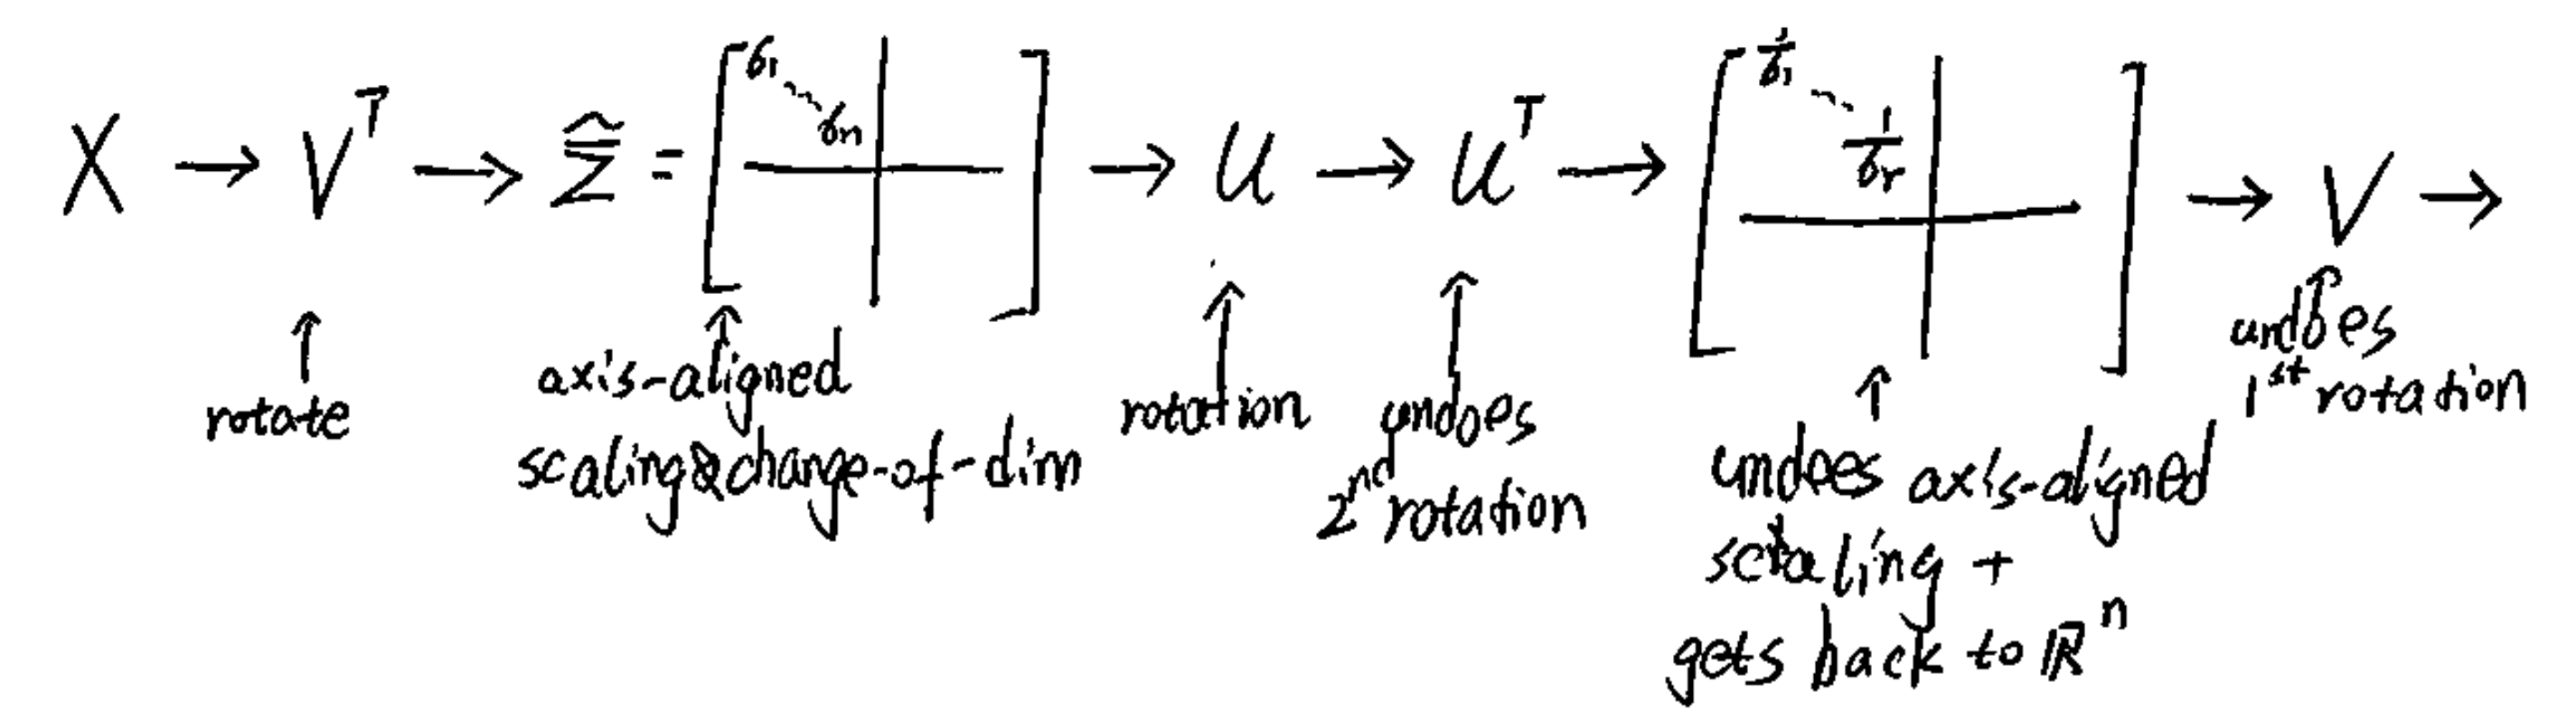
\includegraphics[width=2.1in,height=2.1in]{figures/ch05/figure3.png}
	%\caption{This is an inserted JPG graphic} 
	%\label{fig:graph} 
\end{figure}

\subsection{SVD \& Norms}

\begin{equation*}
||A||^2_F = \sum_i\sum_j a_{ij}^2 = trace(A^TA)
\end{equation*}

\begin{align*}
trace(A^TA) &= trace(V\tilde{\Sigma}\mathcal{U}^T\mathcal{U}\tilde{\Sigma}V^T)\\
&= trace(V\tilde{\Sigma}^T\bar{\Sigma}V^T)\\
&= trace(VV^T\tilde{\Sigma}^T\tilde{\Sigma})\\
&= trace(\tilde{\Sigma}^T\tilde{\Sigma})\\
&= trace(
\begin{bmatrix}%
\Sigma & 0\\
0 & 0
\end{bmatrix}
\begin{bmatrix}%
\Sigma & 0\\
0 & 0
\end{bmatrix})\\
&= trace(
\begin{bmatrix}%
\Sigma^2 & 0\\
0 & 0
\end{bmatrix})\\
&= \sum^r_{i=1}\sigma_i^2 \\
&= ||A||^2_F
\end{align*}
>>>>>>> f279199500e29749d1b0e26d8ab441ab3eae10a9
